\section{Auswertung}
\subsection{Invertierender Linearverstärker}
Zur Untersuchung des invertierenden Linearverstärkers wurden drei Messreihen mit verschiedenen Widerständen im Frequenzbereich $\SIrange{0.01}{1000}{\kilo\hertz}$ aufgenommen. Hierbei wurden jeweils Frequenz $f$, Ausgangsspannung $U_\mathrm{a}$ und zeitliche Differenz $\Delta t$ zwischen den Maxima von Ein- und Ausgangsspannung aufgenommen, welche \autoref{tab:lin_1} bis \ref{tab:lin_3} zu entnehmen sind. Die Widerstandswerte und die sich daraus über \autoref{eqn:verhaeltnis} ergebende theoretische Leerlaufverstärkung sind \autoref{tab:widerstaende} zu entnehmen. Die Eingangsspannung betrug dabei immer $U_\mathrm{e} = \SI{50}{\milli\volt}$.

\begin{table}[H]
  \centering
  \caption{Im Linearverstärker verbaute Widerstände und theoretische Leerlaufverstärkung.}
  \begin{tabular}{c c c c}
    \toprule
    & Messung 1 & Messung 2 & Messung 3\\
    \midrule
    $R_1$/$\si{\kilo\ohm}$ & $\num{1}$ & $\num{1}$ & $\num{15}$\\
    $R_2$/$\si{\kilo\ohm}$ & $\num{100}$ & $\num{150}$ & $\num{100}$\\
    $V_{0,\mathrm{Theo}}$ & $\num{-100}$ & $\num{-150}$ & $-6.\bar{6}$\\
    \bottomrule
  \end{tabular}
  \label{tab:widerstaende}
\end{table}

In \autoref{fig:lin_verstaerkung} sind die aufgenommenen Verstärkungswerte in Abhängigkeit der Frequenz in doppelt logarithmischen Diagrammen für alle Messungen dargestellt.

\begin{figure}[H]
  \centering
  \begin{subfigure}{.4\textwidth}
    \includegraphics[width=\linewidth]{plots/linearverstaerker_1.pdf}
    \subcaption{$R_1 = \SI{1}{\kilo\ohm}$ und $R_2 = \SI{100}{\kilo\ohm}$.}
  \end{subfigure}
  \begin{subfigure}{.4\textwidth}
    \includegraphics[width=\linewidth]{plots/linearverstaerker_2.pdf}
    \subcaption{$R_1 = \SI{1}{\kilo\ohm}$ und $R_2 = \SI{150}{\kilo\ohm}$.}
  \end{subfigure}
  \begin{subfigure}{.4\textwidth}
    \includegraphics[width=\linewidth]{plots/linearverstaerker_3.pdf}
    \subcaption{$R_1 = \SI{15}{\kilo\ohm}$ und $R_2 = \SI{100}{\kilo\ohm}$.}
  \end{subfigure}
  \caption{Verstärkung in Abhängigkeit der Frequenz der Eingangsspannung für die drei Messreihen.}
  \label{fig:lin_verstaerkung}
\end{figure}

Durch das in jedem Plot zu sehende Plateau wird eine konstante Ausgleichsgerade $\log_{10} (V) = b$ gelegt, um die Leerlaufverstärkung des jeweiligen Aufbaus zu ermitteln. Für die drei Messreihen ergeben sich die Werte
\begin{align*}
  b_1 = \num{1.99 \pm 0.012} && b_2 = \num{2.170 \pm 0.0094} && b_3 = \num{1.013 \pm 0.009}.
\end{align*}
Die Leerlaufverstärkung lässt sich dann bestimmen über $V_0 = 10^{b}$, wodurch sich die Werte
\begin{align*}
  V_{0,1} = \num{97 \pm 2.7} && V_{0,2} = \num{148 \pm 3.2} && V_{0,3} = \num{10.3 \pm 0.22}
\end{align*}
ergeben.

Zur Bestimmung der Grenzfrequenz $f_\mathrm{Grenz}$, welche definiert ist als die Frequenz, bei der $V = \frac{1}{\sqrt{2}}$ gilt, wird durch den abfallenden Bereich der Messungen eine Funktion der Form
\begin{equation*}
  \log_{10} (V) = a \cdot \log_{10} (f/\SI{1}{\kilo\hertz}) + b
\end{equation*}
gelegt. Die hierbei ermittelten Parameter lauten
\begin{align*}
  a_1 = \num{-0.86 \pm 0.05} && a_2 = \num{-0.98 \pm 0.05} && a_3 = \num{-0.7 \pm 0.11}\\
  b_1 = \num{2.83 \pm 0.08} && b_2 = \num{3.1 \pm 0.11} && b_3 = \num{2.2 \pm 0.27}.
\end{align*}
Für die Grenzfrequenz gilt durch Umstellen
\begin{equation*}
  f_\mathrm{Grenz}/\SI{1}{\kilo\hertz} = 10^{\frac{\log (\frac{1}{\sqrt{2}}) - b}{a}},
\end{equation*}
woraus sich für die drei Messreihen die Werte
\begin{align*}
  f_{\mathrm{Grenz},1} = \SI{3.1 \pm 1.5 e3}{\kilo\hertz} && f_{\mathrm{Grenz},2} = \SI{2.1 \pm 1.0 e3}{\kilo\hertz} && f_{\mathrm{Grenz},3} = \SI{3 \pm 5 e3}{\kilo\hertz}
\end{align*}
ergeben.
Für das Bandbreitenprodukt ergeben sich hiermit die Werte
\begin{align*}
  B_1 = \num{300758 \pm 146429} && B_2 = \num{312873 \pm 150069} && B_3 = \num{32884 \pm 52863}.
\end{align*}

Die Phasenverschiebung zwischen Ein- und Ausgangsspannung wird berechnet über $\Delta \phi = 2 \pi f \cdot \Delta t$ und ist in Abhängigkeit der Frequenz für alle drei Messreihen in \autoref{fig:phase} aufgetragen.

\begin{figure}[H]
  \centering
  \begin{subfigure}{.4\textwidth}
    \includegraphics[width=\linewidth]{plots/linearverstaerker_phase_1.pdf}
    \subcaption{$R_1 = \SI{1}{\kilo\ohm}$ und $R_2 = \SI{100}{\kilo\ohm}$.}
  \end{subfigure}
  \begin{subfigure}{.4\textwidth}
    \includegraphics[width=\linewidth]{plots/linearverstaerker_phase_2.pdf}
    \subcaption{$R_1 = \SI{1}{\kilo\ohm}$ und $R_2 = \SI{150}{\kilo\ohm}$.}
  \end{subfigure}
  \begin{subfigure}{.4\textwidth}
    \includegraphics[width=\linewidth]{plots/linearverstaerker_phase_3.pdf}
    \subcaption{$R_1 = \SI{15}{\kilo\ohm}$ und $R_2 = \SI{100}{\kilo\ohm}$.}
  \end{subfigure}
  \caption{Phasenverschiebung zwischen Ein- und Ausgangsspannung als Funktion der Frequenz der Eingangsspannung.}
  \label{fig:phase}
\end{figure}
Die Phasenverschiebung $\pi$ bei niedrigen Frequenzen ist Folge der invertierenden Eigenschaft des Linearverstärkers und somit erwartet. Da die Verstärkung bei hohen Frequenzen abnimmt, ist mit einer ansteigenden Phasenverschiebung zu rechnen, allerdings sollte diese gegen $\frac{3\pi}{2}$ laufen, da in dem Fall Eingangs- und Ausgangsspannung destruktiv interferieren würden. Stattdessen läuft die Phasenverschiebung bei hohen Frequenzen in allen Messreihen gegen $2\pi$.

\subsection{Umkehr-Integrator}
Zur Untersuchung des Integrators wurde die Ausgangsspannung $U_\mathrm{a}$ in Abhängigkeit der Frequenz $f$ der Eingangsspannung aufgenommen, wobei es sich bei letzterer um ein sinusförmiges Signal handelt. Hierbei wurden ein Widerstand mit $R = \SI{10}{\kilo\ohm}$ und ein Kondensator mit Kapazität $C = \SI{100}{\nano\farad}$ verwendet. Die Messwerte sind \autoref{tab:int} zu entnehmen und grafisch in \autoref{fig:int_messung} dargestellt.

\begin{figure}[H]
  \centering
  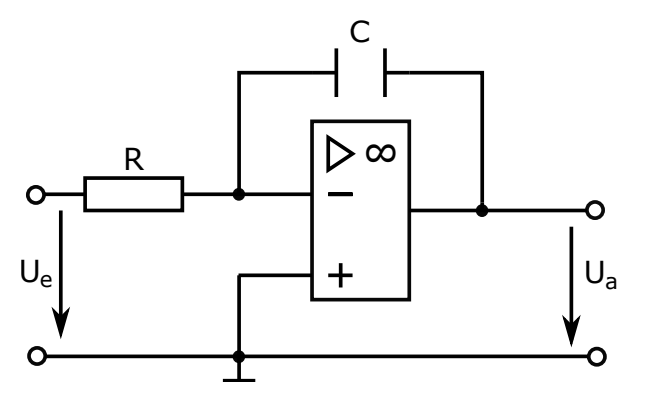
\includegraphics[width=\textwidth]{plots/integrator.pdf}
  \caption{Ausgangsspannung als Funktion der Frequenz an einem Umkehr-Integrator.}
  \label{fig:int_messung}
\end{figure}
Da es sich um einen doppelt-logarithmisches Diagramm handelt, wird der erwartete Zusammenhang zwischen Ein-und Ausgangsspannung zu
\begin{equation*}
  \log_{10} (U_\mathrm{a}/\SI{1}{\volt}) = \log_{10} (- \frac{U_\mathrm{e}}{2\pi R C}/\SI{1}{\volt\per\milli\second}) - \log_{10} (f/\SI{1}{\kilo\hertz}).
\end{equation*}
Zur Überprüfung dieses Zusammenhangs wird durch die aufgenommenen Werte eine Ausgleichsgerade der Form
\begin{equation*}
  \log_{10} (U_\mathrm{a}/\SI{1}{\volt}) = a \cdot \log_{10} (f/\SI{1}{\kilo\hertz}) + b
\end{equation*}
gelegt. Die hierbei erhaltenen Fit-Parameter lauten
\begin{align*}
  a = \num{-1.095 \pm 0.023} && b = \num{-1.560 \pm 0.034}.
\end{align*}
Im Vergleich mit dem erwarteten Zusammenhang lässt sich feststellen, dass $a$ nicht exakt $-1$ beträgt, der Verlauf allerdings in guter Näherung reproduziert werden konnte.

Weiterhin wurde die integrierende Eigenschaft des Integrators anhand eines Dreieck-, Rechteck- und eines Sinus-Signals untersucht. Die dazugehörigen Signale sind \autoref{fig:int_oszi} zu entnehmen, wobei Channel 1 (CH1) das jeweilige Ausgangs- und Channel 2 (CH2) das jeweilige Eingangssignal zeigt.

\begin{figure}[H]
  \centering
  \begin{subfigure}{.4\textwidth}
    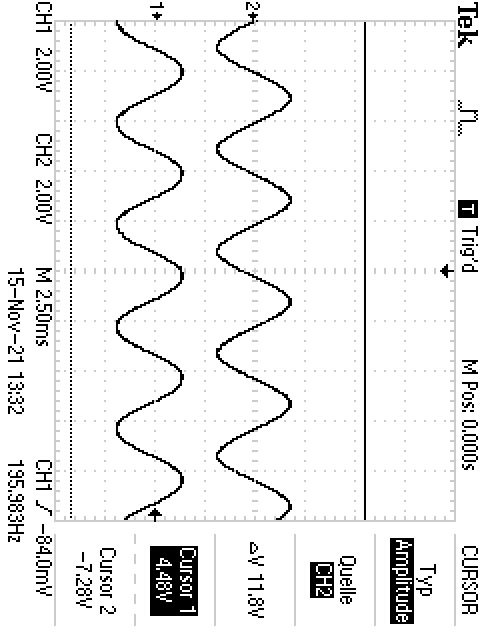
\includegraphics[width=\linewidth]{data/ALL0059/F0059TEK.JPG}
    \subcaption{Das Integral einer Sinus-Spannung.}
  \end{subfigure}
  \begin{subfigure}{.4\textwidth}
    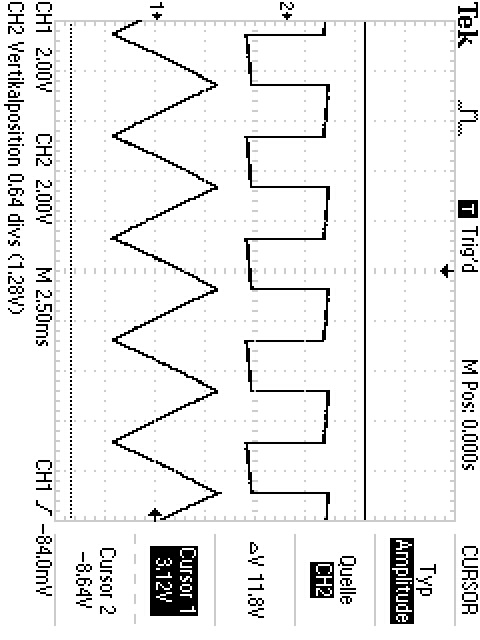
\includegraphics[width=\linewidth]{data/ALL0060/F0060TEK.JPG}
    \subcaption{Das Integral einer Rechteck-Spannung.}
  \end{subfigure}
  \begin{subfigure}{.4\textwidth}
    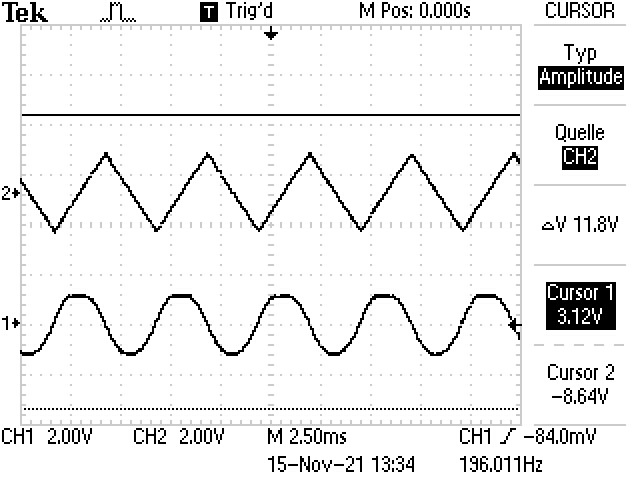
\includegraphics[width=\linewidth]{data/ALL0061/F0061TEK.JPG}
    \subcaption{Das Integral einer Dreieck-Spannung.}
  \end{subfigure}
  \caption{Ein- und Ausgangssignale des Integrators für verschiedene Eingangsspannungen.}
  \label{fig:int_oszi}
\end{figure}

Das Integral einer Rechteck-Spannung ist eine Dreieck-Spannung, das der Dreieck-Spannung eine Parabel und das einer Sinus-Funktion ein Cosinus. All diese Integrale sind auch auf dem Oszilloskop zu sehen. Die integrierende Funktion des Integrators konnte also bestätigt werden.

\subsection{Invertierender Differenzierer}
Zur Untersuchung des invertierenden Differenzierers wird analog zum vorherigen Abschnitt vorgegangen. Dabei wurden ein Widerstand mit $R = \SI{100}{\kilo\ohm}$ und ein Kondensator mit Kapazität $C = \SI{22}{\nano\farad}$ verwendet. Die aufgenommenen Messwerte sind \autoref{tab:diff} zu entnehmen und grafisch in \autoref{fig:diff_messung} dargestellt.

\begin{figure}[H]
  \centering
  \includegraphics[width=\textwidth]{plots/differenzierer.pdf}
  \caption{Ausgangsspannung als Funktion der Frequenz bei einem Differenzierer.}
  \label{fig:diff_messung}
\end{figure}

Da es sich um einen doppelt-logarithmischen Plot handelt, wird aus dem Zusammenhang zwischen Ein- und Ausgangsspannung bei einem Sinus-Signal
\begin{equation*}
  \log_{10} (U_\mathrm{a}/\SI{1}{\volt}) = \log_{10} (f/\SI{1}{\kilo\hertz}) + \log_{10} (- 2 \pi R C U_\mathrm{e}/\SI{1}{\volt\micro\second}).
\end{equation*}
Zur Überprüfung dieses Zusammenhangs wird analog zum Integrator eine Ausgleichsgerade durch die Messwerte gelegt, wobei sich die Parameter
\begin{align*}
  a = \num{1.0022 \pm 0.0032} && b = \num{2.838 \pm 0.005}
\end{align*}
ergeben. Folglich lässt sich der theoretische Zusammenhang zwischen Ausgangsspannung und Frequenz experimentell bestätigen.

Weiterhin wurden zur Überprüfung der differenzierenden Eigenschaft des invertierenden Differenzierers Ein- und Ausgangssignale am Oszilloskop untersucht. Die aufgenommenen Bilder sind \autoref{fig:diff_oszi} zu entnehmen.

\begin{figure}[H]
  \centering
  \begin{subfigure}{.4\textwidth}
    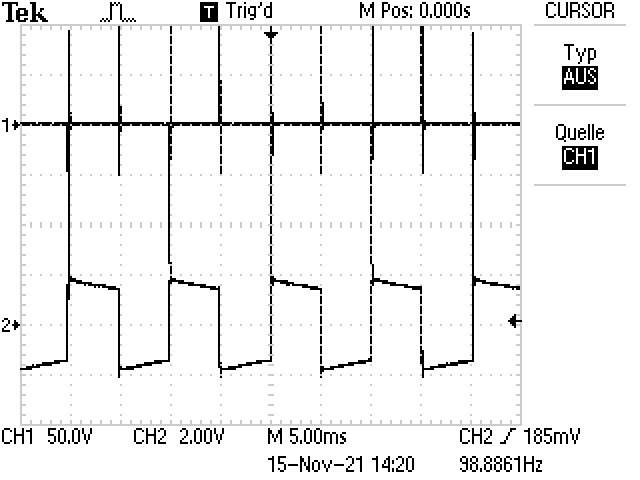
\includegraphics[width=\linewidth]{data/ALL0062/F0062TEK.JPG}
  \end{subfigure}
  \begin{subfigure}{.4\textwidth}
    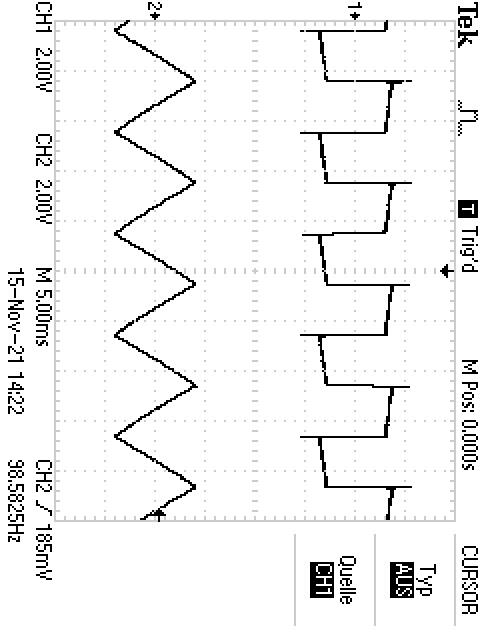
\includegraphics[width=\linewidth]{data/ALL0063/F0063TEK.JPG}
  \end{subfigure}
  \begin{subfigure}{.4\textwidth}
    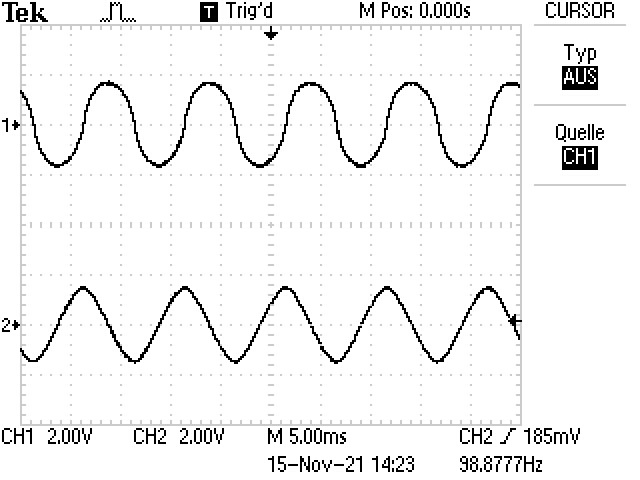
\includegraphics[width=\linewidth]{data/ALL0064/F0064TEK.JPG}
  \end{subfigure}
  \caption{Ein- und Ausgangsspannung eines Differenzierers für ein Dreieck- (links), Rechteck- (mitte) und Sinus-Eingangssignal (rechts).}
  \label{fig:diff_oszi}
\end{figure}


Bei einer Dreieck-Spannung als Eingangsspannung wird eine Rechteck-Spannung als Ausgangsspannung erwartet, bei einer Rechteck-Spannung als Eingangsspannung wird eine konstante Spannung von $\SI{0}{\volt}$ erwartet und bei einem Sinus-Eingangssignal wird als Ausgang ein Cosinus erwartet. Diese Zusammenhänge konnten folglich bestätigt werden, wobei an den Unstetigkeiten das Gibb'sche Phänomen zu beobachten ist.

\subsection{Nicht-invertierender Schmitt-Trigger}

Zur Untersuchung des Nicht-invertierenden Schmitt-Triggers werden die Widerstände $R_1 = \SI{10}{\kilo\ohm}$ und $R_2 = \SI{220}{\kilo\ohm}$ verbaut. Die Kipp-Spannung wurde bei $U_{\mathrm{e, Kipp}} = \SI{680}{\milli\volt}$ gefunden. In \autoref{fig:schmitt_oszi} ist der Verlauf der Ein- und Ausgangsspannung am Oszilloskop dargestellt.

\begin{figure}[H]
  \centering
  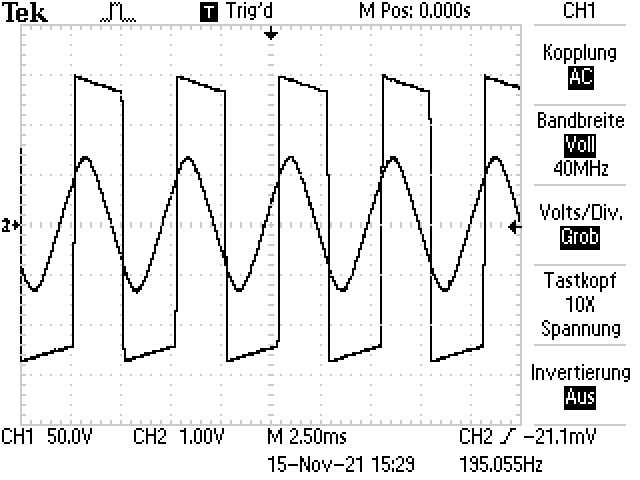
\includegraphics{data/ALL0066/F0066TEK.JPG}
  \caption{Oszilloskop-Bild des Schmitt-Triggers, wobei CH1 das Ausgangs- und CH2 das Eingangssignal zeigt.}
  \label{fig:schmitt_oszi}
\end{figure}

Der theoretische Wert beträgt $U_{S_{\pm}} = \SI{0.68181}{\volt}$.

\subsection{Signalgenerator}
In \autoref{fig:signalgenerator_oszi} ist der Spannungsverlauf der Eingangsspannung und der Ausgangsspannung an einem Signalgenerator zu sehen.

\begin{figure}[H]
  \centering
  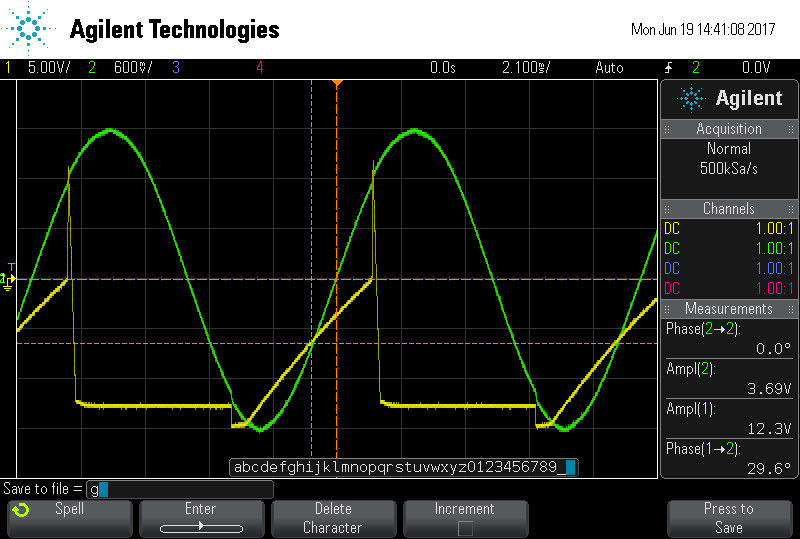
\includegraphics[width=\textwidth]{signalgen.png}
  \caption{Ein- (grün) und Ausgangssignal (gelb) an einem Signalgenerator.}
  \label{fig:signalgenerator_oszi}
\end{figure}
Am aufsteigenden Ast der Ausgangsspannung ist wie zu erwarten ein Dreieck-Signal zu erkennen. Der abfallende Ast hingegen besteht vor Allem aus Unstetigkeiten und einem Rechteck-Signal. Hier versagt folglich der Integrator.
